% !TeX root = ../Document.tex
\documentclass[../Document.tex]{subfiles}

\begin{document}
\section{A4988} \label{acdoo}
Upravljač motora A4988 je namijenjen za upravljanje bipolarnim koračnim motorima\cite{adriver}. Pomoću ovog uređaja, motoru motožemo dostaviti i do 2A po namotaju. Međutim, za jačinu struje se ne moramo previše brinuti jer A4988 ima ugrađenu zaštitu od prekomjerne jačine struje (eng. overcurrent protection).

\subsection{Digitalno-analogni konverter}
U elektronici se dizajneri često susreću sa situacijom da je iz digitalnog potrebno dobiti analogni signal. Ovaj problem se riješava koristeći digitalno-analogne konvertere (eng. Digital-to-analog converter, DAC)\cite{dac}.
\cFigure{A4988_DAC}{8-bitni DAC}{0.7}

DAC funkcioniše tako što konvertuje abstraktni broj konačne preciznosti u analogni signal čija je voltaža proporcionalna ulaznoj vrijednosti. Idealan DAC konvertuje abstraktni broj u niz impulsa, nakon čega se, koristći linearnu interpolaciju, popunjava signal između impulsa.
\cFigure{A4988_DAC-Signal}{Primjer idealne konverzije iz digitalnog u analogni signal}{0.5}

\subsection{H-most}
H-most je električno kolo čijij je zadatak kontrola toka struje. Najčešće se pojavljuju kao već integrisane komponente. H-most je građen iz četiri prekidača čijim se kombiniranjem u motoru mijenja tok struje.

\cFigure{A4988_H-Most}{H-most}{0.5}

H-most ima dva moda u kojima prekidači mogu biti postavljeni, a to su brzo i sporo propadanje (eng. decay). U ovom kontekstu, propadanje prestavlja brzinu kojom se jačina struje u navoju može spustiti na 0.

\begin{figure}
    \centering
    \subfloat[Brzo propradanje]{{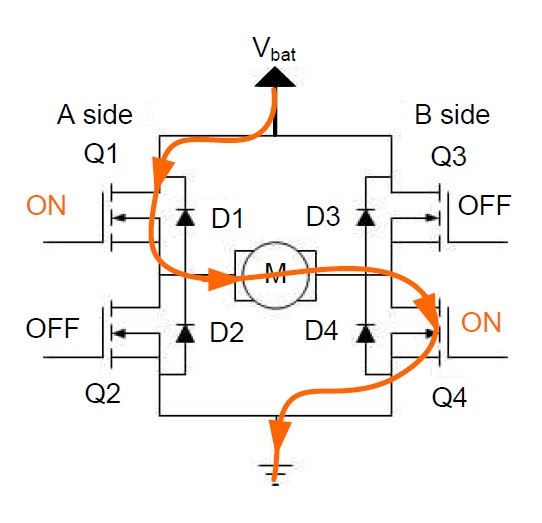
\includegraphics[width=0.3\textwidth]{A4988_Fast-Decay} }}
    \qquad
    \subfloat[Sporo propadanje]{{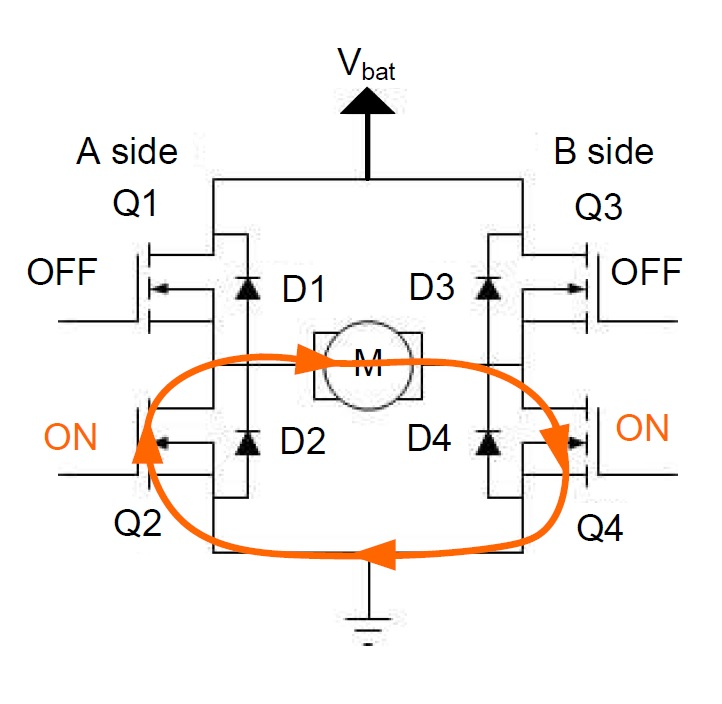
\includegraphics[width=0.3\textwidth]{A4988_Slow-Decay} }}
    \caption{Modovi rada H-mosta}
\end{figure}

\subsection{Miješano propadanje}
U svakom koraku motora, protok struje se kontrolira koristeći vrijednost eksternih rezistora čija je uloga opažati ulazni protok struje, referentnu voltažu i izlaznu voltažu digitalno-analognog konvertera koja se kontroliše od strane translatora. Ukoliko je trenutni izlaz DAC-a u niži u odnosu na prošli, onda se mod aktivnog mosta postavlja na mod miješanog propadanja (jedno od svojstava A4988 čipa). Ukoliko je trenutni izlaz DAC-a viši, postavlja se na sporo propadanje. Ovo dinamično mijenjanje modova poboljšava performanse motora u vidu smanjenja distorzije talasa koji prenosi signal\cite{adriver}.

\subsection{Pinovi} \label{apinovi}
A4988 upravljač, na sebi ima 16 pinova:

\subparagraph{ENABLE} \noindent se koristi za privremeno isključenje uređaja. Kada se na njemu nalazi visoki nivo voltaže, uređaj neće primati naredbe.

\subparagraph{MS1, MS2, MS3} \noindent su pinovi koji određuju rezoluciju mikrokoračanja motora. Šablonskim potavljenjem visokog voltažnog nivoa, upravljač će način rada prebaciti na drugi mikrokoračni mod. \label{microstepping}


\begin{table}[h]
    \centering
    \begin{tabular}{ |c|c|c|c| }
        \hline
        MS1 & MS2 & MS3 & Rezolucija u veličini koraka \\
        \hline
        N   & N   & N   & \sfrac{1}{1}                 \\
        \hline
        V   & N   & N   & \sfrac{1}{2}                 \\
        \hline
        N   & V   & N   & \sfrac{1}{4}                 \\
        \hline
        V   & V   & N   & \sfrac{1}{8}                 \\
        \hline
        V   & V   & V   & \sfrac{1}{16}                \\
        \hline
    \end{tabular}
    \caption{Šabloni MS pinova\cite{adriver}}
\end{table}

\subparagraph{RESET} \noindent vraća translator na početno stanje. Dok je na njemu visoki nivo voltaže, svi ulazi se ignorišu.

\subparagraph{SLEEP} \noindent se koristi za uštedu energije i postavljajući na njega visoki nivo voltaže, uređaj se stavlja u ``sleep mode''.

\subparagraph{STEP} \noindent pin - slanjem impulsa voltaže visokog nivoa na ovaj pin ,a zatim vraćanjem istog na niski nivo voltaže, upravljač pravi jedan korak na motoru u smjeru zavisnom od stanja DIR pina i veličine zavisne od trenutne rezolucije.

\subparagraph{DIR} \noindent služi za određivanje smjera u kojem će se osa motora okretati. Ovaj pin mora konstantno imati na sebe pušten nivo voltaže gdje visoki i niski određuju smjer.

\subparagraph{VMOT}\label{a4988pow} \noindent je ulaz za struju kojom će se napajati motor. Voltaža ove struje treba biti između 8V i 35V.

\subparagraph{VDD} \noindent predstavlja zvor struje za upravljač.

\subparagraph{GND} \noindent - na upravljaču se nalaze 2 pina za uzemljenje, jedan za struju koja napaja sam uređaj, drugi za struju koja napaja motore.

\subparagraph{1A,1B,2A,2B} \noindent su pinovi koji se povezuju direktno na motor. Parovi za navoje su 2A i 2B, kao i 1A i 1B.

\cFigure{A4988_Pinovi}{Najjednostavnija šema spajanja A9488}{0.6}

\subsection{Specifikacije}

\begin{table}[h]
    \centering
    \begin{tabular}{ |c|c| }
        \hline
        Potrebna struja          & 3V-5V                                 \\
        \hline
        Maksimalna jačina struje & 2A                                    \\
        \hline
        Termalno gašenje         & -20{\textdegree}C, + 80{\textdegree}C \\
        \hline
        Dužina                   & do 20.3mm                             \\
        \hline
        Širina                   & do 15.2mm                             \\
        \hline
    \end{tabular}
    \caption{A4988 specifikacije}
\end{table}

\noindent A4988 na sebi ima potenciometar kojim se može kontrolisati jačina struje koja prolazi kroz upravljač.

\end{document}